% Grobe  Architekturbeschreibung  durch  Bausteine/Komponenten  (Kein  detailliertes Klassendiagramm).

Das Projekt soll aus drei separaten Programmen bestehen. Es soll dabei keine Kommunikation untereinander stattfinden. Stattdessen greifen alle auf eine gemeinsame Datenbank zu. Eine Darstellung der drei Komponenten ist in Abbildung~\ref{c:systemmodell} zu finden.

\begin{figure}[h]
	\centering
	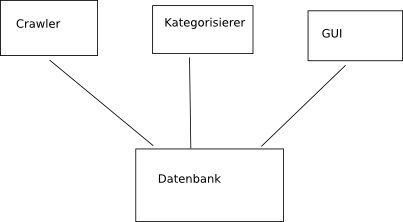
\includegraphics{img/systemmodell.png}
	\caption{Das Systemmodell}
	\label{c:systemmodell}
\end{figure}

\begin{description}
	\item[Crawler] Aufgabe des Crawlers ist es mithilfe der Twitter-Streaming-API die Twitterdaten zu sammeln. Es sollen verifizierte Benutzer und Retweets von Tweets dieser Nutzer gefunden werden. Diese Daten sollen noch im Crawler lokalisiert werden, bevor sie in der Datenbank abgespeichert werden.
	\item[Kategorisierer] Um den Crawler so leichtgewichtig wie möglich zu halten, werden die gefunden Accounts von einer weiteren Anwendung, dem Kategorisierer kategorisiert. Unabhängig vom Crawler sucht er in der Datenbank nach Accounts, denen noch keine Kategorie zugeordnet wurde. Anhand der Daten aus der DMOZ-Datenbank sollen diese Accounts dann hierarchisch kategorisiert werden. Dabei können einem Nutzer mehrere Kategorien zugeordnet werden. Der Kategorisierer arbeitet also auf den vom Crawler gefunden Daten und vervollständigt diese.
	\item[GUI] Die GUI greift lesend und eingeschränkt schreibend auf die Datenbank zu und visualisiert die Daten anhand vom Nutzer gegebener Eingaben. Sie baut somit auf Crawler und Kategorisierer auf, welche jedoch unabhängig von der GUI sind. Es ist möglich über die GUI weitere Twitteraccounts (auch nicht verifizierte) in die Datenbank aufzunehmen. Dies ist die einzige Art der Kommunikation von der GUI zur Datenbank.
\end{description}


